\documentclass[tikz,border=10pt]{standalone}
\usepackage{amsmath,amssymb}
\usepackage{tikz}
\usetikzlibrary{arrows,automata,backgrounds,calendar,chains,decorations,decorations.pathreplacing,decorations.text,fit,matrix,mindmap,patterns,petri,plotmarks,positioning,shadows,shapes,shapes.callouts,shapes.geometric,shapes.misc,spy,trees,calc,intersections,tikzmark,arrows.meta}
\usepackage{xcolor}
\usepackage{pgfplots}
\pgfplotsset{compat=1.16}

% Common math macros from the book
\def\x{\mathbf{x}}
\def\y{\mathbf{y}}
\def\z{\mathbf{z}}
\def\A{\mathbf{A}}
\def\b{\mathbf{b}}
\def\c{\mathbf{c}}
\def\w{\mathbf{w}}
\def\v{\mathbf{v}}
\def\u{\mathbf{u}}
\def\e{\mathbf{e}}
\def\zero{\mathbf{0}}
\def\R{\mathbb{R}}
\def\N{\mathbb{N}}
\def\Z{\mathbb{Z}}
\def\Q{\mathbb{Q}}
\def\st{\text{s.t.}}
\def\vect#1{\mathbf{#1}}
\def\xLP{x^{\mathrm{LP}}}
\def\zLP{z^{\mathrm{LP}}}
\def\xIP{x^{\mathrm{IP}}}

% Common node styles from the book
\tikzset{
    main/.style={circle, draw, fill=gray!20, minimum size=1cm, font=\normalsize},
    dot/.style={circle,fill=blue,minimum size=3pt,inner sep=0pt, outer sep=-1pt},
    vertex/.style={circle,fill=black!25,minimum size=20pt,inner sep=0pt},
    edge/.style={draw,-,thick},
    directed edge/.style={draw,->,>=latex,thick},
}

% Additional macros for 3D/coordinate systems
\newcommand{\xhat}{\hat{\x}}
\newcommand{\yhat}{\hat{\y}}
\newcommand{\zhat}{\hat{\z}}
\newcommand{\ihat}{\hat{\imath}}
\newcommand{\jhat}{\hat{\jmath}}
\newcommand{\khat}{\hat{k}}

\begin{document}
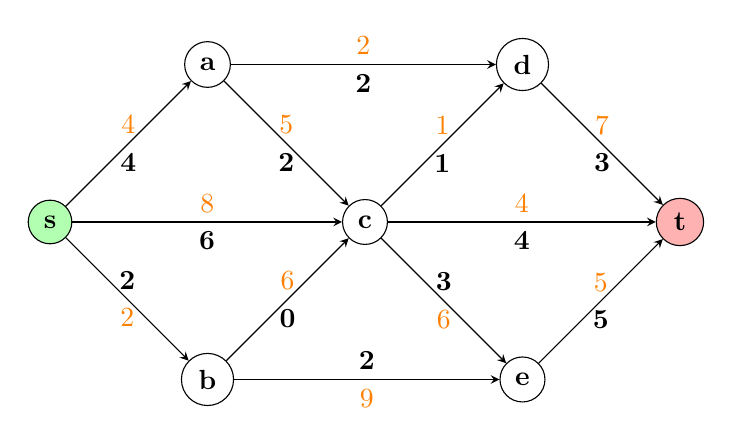
\begin{tikzpicture}[>=stealth, node distance=2cm]

    % Nodes with specific styles
    \node[draw, circle, fill=green,
         fill opacity = 0.3,  text opacity=1] (s) at (0,2) {\textbf{s}};
    \node[draw, circle] (a) at (2,4) {\textbf{a}};
    \node[draw, circle] (b) at (2,0) {\textbf{b}};
    \node[draw, circle] (c) at (4,2) {\textbf{c}};
    \node[draw, circle] (d) at (6,4) {\textbf{d}};
    \node[draw, circle] (e) at (6,0) {\textbf{e}};
    \node[ fill=red,
         fill opacity = 0.3, draw, circle,  text opacity=1] (t) at (8,2) {\textbf{t}};

    % Edges with costs (orange, upright) and flows (bold black, below)
    \draw[->] (s) -- (a) node[midway, above, text=orange] {4} 
                         node[midway, below, text=black] {\textbf{4}};
    \draw[->] (s) -- (c) node[midway, above, text=orange] {8} 
                         node[midway, below, text=black] {\textbf{6}};
    \draw[->] (s) -- (b) node[midway, below, text=orange] {2} 
                         node[midway, above, text=black] {\textbf{2}};
    
    \draw[->] (a) -- (c) node[midway, above, text=orange] {5} 
                         node[midway, below, text=black] {\textbf{2}};
    \draw[->] (a) -- (d) node[midway, above, text=orange] {2} 
                         node[midway, below, text=black] {\textbf{2}};

    \draw[->] (c) -- (d) node[midway, above, text=orange] {1} 
                         node[midway, below, text=black] {\textbf{1}}; % Adjusted to respect capacity
    \draw[->] (c) -- (t) node[midway, above, text=orange] {4} 
                         node[midway, below, text=black] {\textbf{4}};
    \draw[->] (c) -- (e) node[midway, below, text=orange] {6} 
                         node[midway, above, text=black] {\textbf{3}};

    \draw[->] (b) -- (c) node[midway, above, text=orange] {6} 
                         node[midway, below, text=black] {\textbf{0}};
    \draw[->] (b) -- (e) node[midway, below, text=orange] {9} 
                         node[midway, above, text=black] {\textbf{2}};

    \draw[->] (d) -- (t) node[midway, above, text=orange] {7} 
                         node[midway, below, text=black] {\textbf{3}};
    \draw[->] (e) -- (t) node[midway, above, text=orange] {5} 
                         node[midway, below, text=black] {\textbf{5}};

\end{tikzpicture}
\end{document}
